\documentclass[12pt]{beamer}

\usepackage{préambule}

\renewcommand{\arraystretch}{1.3}

\begin{document}

\begin{frame}
	\begin{center}
		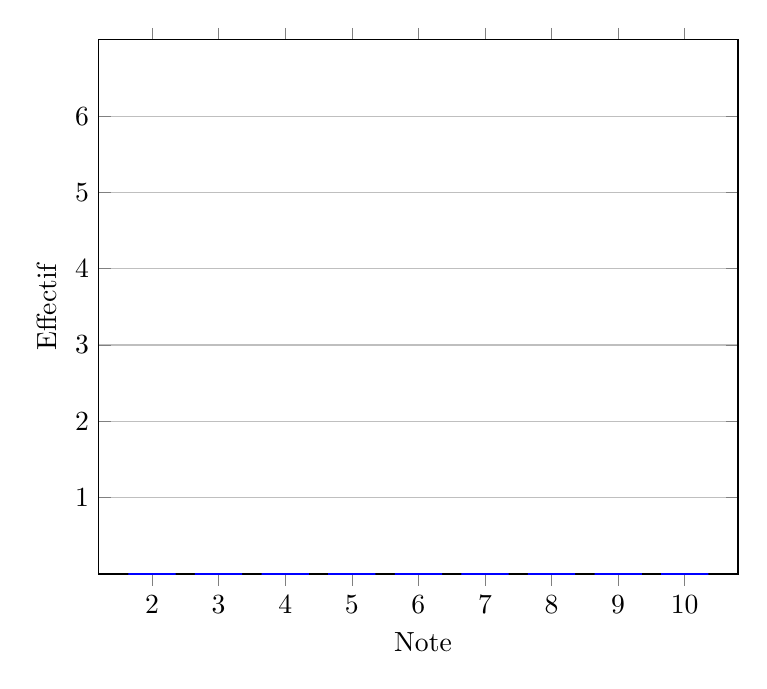
\begin{tikzpicture}
			\begin{axis}[
					width = 0.8\textwidth,
					ybar,
					bar width=0.6cm,
					ymin=0, ymax=7,
					ylabel={Effectif},
					xlabel={\ Note},
					symbolic x coords={2, 3, 4, 5, 6, 7, 8, 9, 10},
					xtick=data,
					ymajorgrids = true,
					scaled y ticks = false,
					ytick={1,2,3,4,5,6},
				]
				\addplot coordinates { (2,0) (3,0) (4,0) (5,0) (6,0) (7,0) (8,0) (9,0) (10,0) };
			\end{axis}
		\end{tikzpicture}
	\end{center}
\end{frame}

\begin{frame}
	\begin{center}
		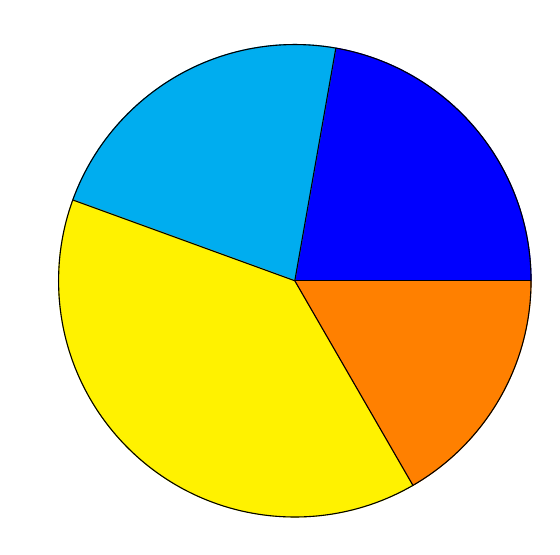
\begin{tikzpicture}
			\coordinate (P1) at (3,0);
			\coordinate (P2) at (0.5209445330007912,2.954423259036624);
			\coordinate (P3) at (-2.819077862357725,1.0260604299770066);
			\coordinate (P4) at (1.5000000000000004,-2.598076211353316);
			\filldraw[color=blue] (0,0) -- (P1) arc (0:80:3);
			\filldraw[color=cyan] (0,0) -- (P2) arc (80:160:3);
			\filldraw[color=yellow] (0,0) -- (P3) arc (160:300:3);
			\filldraw[color=orange] (0,0) -- (P4) arc (300:360:3);
			\draw (0,0) circle (3);
			\draw (0,0) -- (3,0);
			\draw (0,0) -- (P2);
			\draw (0,0) -- (P3);
			\draw (0,0) -- (P4);
		\end{tikzpicture}
	\end{center}
\end{frame}

\begin{frame}
	\begin{center}
		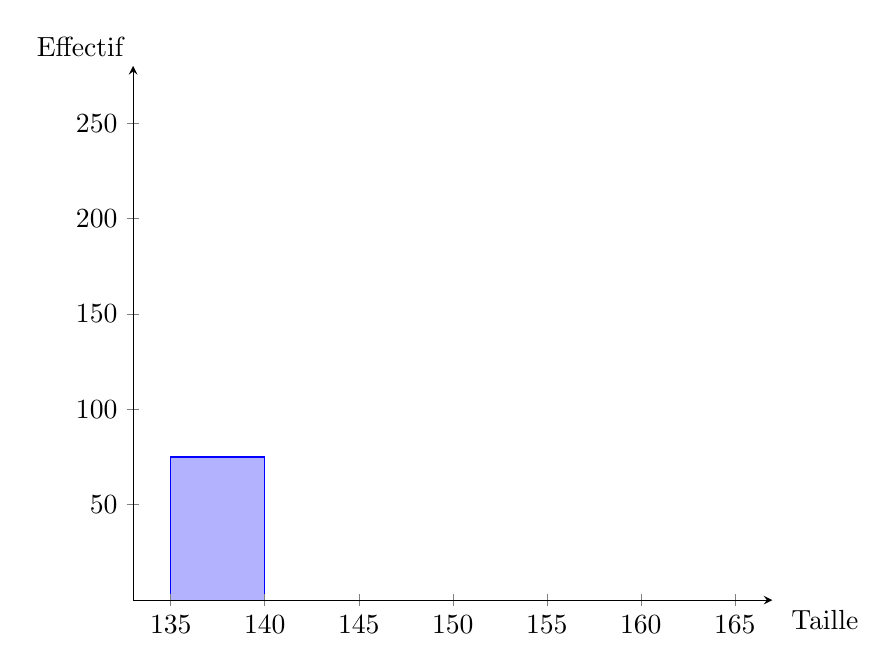
\begin{tikzpicture}
			\begin{axis}[
					width = 0.8\textwidth,
					xmin=133, xmax=167,
					ymin=0, ymax=280,
					axis lines=center,
					ylabel={Effectif},
					xlabel={\ Taille},
					xlabel style={below right},
					ylabel style={above left},
					area style,
					xtick={135,140,145,150,155,160,165}
				]
				\addplot+[ybar interval,mark=no] plot coordinates { (135,75) (140, 0) };
			\end{axis}
		\end{tikzpicture}
	\end{center}
\end{frame}

\end{document}